% $Id: template.tex 11 2007-04-03 22:25:53Z jpeltier $

\documentclass{vgtc}                          % final (conference style)
%\documentclass[review]{vgtc}                 % review
%\documentclass[widereview]{vgtc}             % wide-spaced review
%\documentclass[preprint]{vgtc}               % preprint
%\documentclass[electronic]{vgtc}             % electronic version

%% Uncomment one of the lines above depending on where your paper is
%% in the conference process. ``review'' and ``widereview'' are for review
%% submission, ``preprint'' is for pre-publication, and the final version
%% doesn't use a specific qualifier. Further, ``electronic'' includes
%% hyperreferences for more convenient online viewing.

%% Please use one of the ``review'' options in combination with the
%% assigned online id (see below) ONLY if your paper uses a double blind
%% review process. Some conferences, like IEEE Vis and InfoVis, have NOT
%% in the past.

%% Figures should be in CMYK or Grey scale format, otherwise, colour 
%% shifting may occur during the printing process.

%% These few lines make a distinction between latex and pdflatex calls and they
%% bring in essential packages for graphics and font handling.
%% Note that due to the \DeclareGraphicsExtensions{} call it is no longer necessary
%% to provide the the path and extension of a graphics file:
%% \includegraphics{diamondrule} is completely sufficient.
%%
\ifpdf%                                % if we use pdflatex
  \pdfoutput=1\relax                   % create PDFs from pdfLaTeX
  \pdfcompresslevel=9                  % PDF Compression
  \pdfoptionpdfminorversion=7          % create PDF 1.7
  \ExecuteOptions{pdftex}
  \usepackage{graphicx}                % allow us to embed graphics files
  \DeclareGraphicsExtensions{.pdf,.png,.jpg,.jpeg} % for pdflatex we expect .pdf, .png, or .jpg files
\else%                                 % else we use pure latex
  \ExecuteOptions{dvips}
  \usepackage{graphicx}                % allow us to embed graphics files
  \DeclareGraphicsExtensions{.eps}     % for pure latex we expect eps files
\fi%

%% it is recomended to use ``\autoref{sec:bla}'' instead of ``Fig.~\ref{sec:bla}''
\graphicspath{{figures/}{pictures/}{images/}{./}} % where to search for the images

\usepackage[utf8]{inputenc}
\usepackage[english]{babel}
\usepackage{microtype}                 % use micro-typography (slightly more compact, better to read)
\PassOptionsToPackage{warn}{textcomp}  % to address font issues with \textrightarrow
\usepackage{textcomp}                  % use better special symbols
\usepackage{mathptmx}                  % use matching math font
\usepackage{times}                     % we use Times as the main font
\renewcommand*\ttdefault{txtt}         % a nicer typewriter font
\usepackage{cite}                      % needed to automatically sort the references
\usepackage{tabu}                      % only used for the table example
\usepackage{booktabs}                  % only used for the table example
\usepackage{hyperref}
%% We encourage the use of mathptmx for consistent usage of times font
%% throughout the proceedings. However, if you encounter conflicts
%% with other math-related packages, you may want to disable it.


%% If you are submitting a paper to a conference for review with a double
%% blind reviewing process, please replace the value ``0'' below with your
%% OnlineID. Otherwise, you may safely leave it at ``0''.
\onlineid{0}

%% declare the category of your paper, only shown in review mode
\vgtccategory{Research}

%% allow for this line if you want the electronic option to work properly
\vgtcinsertpkg

%% In preprint mode you may define your own headline.
%\preprinttext{To appear in an IEEE VGTC sponsored conference.}

%% Paper title.

\title{Global Illumination for Fun and Profit}

%% This is how authors are specified in the conference style

%% Author and Affiliation (single author).
%%\author{Roy G. Biv\thanks{e-mail: roy.g.biv@aol.com}}
%%\affiliation{\scriptsize Allied Widgets Research}

%% Author and Affiliation (multiple authors with single affiliations).
%%\author{Roy G. Biv\thanks{e-mail: roy.g.biv@aol.com} %
%%\and Ed Grimley\thanks{e-mail:ed.grimley@aol.com} %
%%\and Martha Stewart\thanks{e-mail:martha.stewart@marthastewart.com}}
%%\affiliation{\scriptsize Martha Stewart Enterprises \\ Microsoft Research}

%% Author and Affiliation (multiple authors with multiple affiliations)
\author{Felipe Nunes Walmsley\thanks{e-mail: fnw@cin.ufpe.br}\\ %
        \scriptsize Centro de Informática - UFPE %
}

%% A teaser figure can be included as follows, but is not recommended since
%% the space is now taken up by a full width abstract.
%\teaser{
%  \includegraphics[width=1.5in]{sample.eps}
%  \caption{Lookit! Lookit!}
%}

%% Abstract section.
\abstract{
	Over the years, several attempts have been made to assess the quality of higher education in Brazil. Currently, the ENADE exam is one of the most important tools in this assessment, and detailed data about exam results are made available to the public. We propose a visualization tool aimed at revealing regional differences in students performance, focusing on mean scores, and relative percentages of top and bottom scorers. Our results show clear regional differences, and suggest that factors within a state can heavily influence the performance of students, specially when compared to neighboring states. 
} % end of abstract

%% ACM Computing Classification System (CCS). 
%% See <http://www.acm.org/about/class> for details.
%% We recommend the 2012 system <http://www.acm.org/about/class/class/2012>
%% For the 2012 system use the ``\CCScatTwelve'' which command takes four arguments.
%% The 1998 system <http://www.acm.org/about/class/class/2012> is still possible
%% For the 1998 system use the ``\CCScat'' which command takes four arguments.
%% In both cases the last two arguments (1998) or last three (2012) can be empty.

\CCScatlist{
  \CCScatTwelve{Human-centered computing}{Visu\-al\-iza\-tion}{Visu\-al\-iza\-tion techniques}{};
}

%\CCScatlist{
  %\CCScat{H.5.2}{User Interfaces}{User Interfaces}{Graphical user interfaces (GUI)}{};
  %\CCScat{H.5.m}{Information Interfaces and Presentation}{Miscellaneous}{}{}
%}

%% Copyright space is enabled by default as required by guidelines.
%% It is disabled by the 'review' option or via the following command:
% \nocopyrightspace

%%%%%%%%%%%%%%%%%%%%%%%%%%%%%%%%%%%%%%%%%%%%%%%%%%%%%%%%%%%%%%%%
%%%%%%%%%%%%%%%%%%%%%% START OF THE PAPER %%%%%%%%%%%%%%%%%%%%%%
%%%%%%%%%%%%%%%%%%%%%%%%%%%%%%%%%%%%%%%%%%%%%%%%%%%%%%%%%%%%%%%%%

\begin{document}

%% The ``\maketitle'' command must be the first command after the
%% ``\begin{document}'' command. It prepares and prints the title block.

%% the only exception to this rule is the \firstsection command
\firstsection{Introduction}



\maketitle

In education, there is a constant concern with measuring the performance of students, and in particular there is a desire to use these measures to assess the quality of the education being provided to students. In Brazil, there are several initiatives designed to measure the performance of students at each level of education, such as the mandatory exams:

\begin{itemize}
	\item{The \emph{Prova Brasil}, designed to measure the performance of primary school students;}
	\item{The National Secondary Education Exam (from the Portuguese \emph{Exame Nacional do Ensino Médio}, ENEM), aimed at secondary students;}
	\item{The National Students Performance Exam (from the Portuguese \emph{Exame Nacional de Desempenho dos Estudantes}, ENADE), which assesses tertiary education.}
\end{itemize}

This last exam is the focus of this work. The (INEP), an institute subject to the Brazilian Ministry of Education publishes a data set containing the results of the exam, down to the level of individual students. This provides us with a unique opportunity to perform a number of analyses, which can help us paint a detailed picture of the current state of tertiary education in Brazil, and whether not the students are achieving the (formação) expected of them, and what factors are contributing to or detracting from their education. 

While there are previous work dealing with ENADE, these consist mostly of research in the field of education. The works in \cite{brito2008sinaes} and \cite{verhine2006provao} deal with ENADE from a historical and conceptual perspective. There are very few work that deal with the micro-data itself. In \cite{vista2017tecnicas
}, the authors perform data mining to discover patterns on the 2014 exam data set, but the analysis is restricted to Computer Science programs in the state of Rio Grande do Sul. To the best of our knowledge, there is no work directly comparable to ours using ENADE data in the field of visualization. 

In this work, we propose a visualization tool, which aims to help the user tease out interesting patterns in the distribution of students' grades around the country. The tool focuses on highlighting regional differences, allowing the user to observe how the students of each state perform, and also how unequal is the performance of students within each state. 



\section{Background and Related Works}

\subsection{The ENADE exam}

In Brazil, the Ministry of Education requires all first and last year university students to sit in the ENADE. This exam aims to assess the knowledge of the students in both general topics and in their area of study, as a means to ascertain the quality of tertiary education in Brazil. The exam is applied in a rotating fashion to students from different areas of knowledge.

The individual (but anonymized) results for each student are made publicly available \cite{enadedados}. The data set contains detailed information about each student, such as their answers to individual items in the exam, their grades in the general and specific portions of the exams, and their overall grade. The 2016 ENADE micro-data data set consists of 216044 entries, each with 141 variables.

Furthermore, the students are required to answer a comprehensive questionnaire, which queries the students in relation to topics such as their perception of the exam itself, their opinion about the quality of their college and program, and also questions about their socioeconomic background. Below, some examples of the types of questions presented in the questionnaire, translated from the Portuguese original.

\begin{itemize}
	\item{\emph{Perception of the exam:} How hard was this exam in the general knowledge portion?}
	\item{\emph{Opinion about their college/program:} Are the labs, equipment and materials available to your program adequate to the needs of the program? }
	\item{\emph{Socioeconomic background:} Was your admission to the university due to affirmative action policies?}
\end{itemize}

Given the plethora of data available, a multitude of analysis are possible. In fact, the data set is so large and complex that any single work would be incapable of performing a satisfactorily comprehensive analysis of the data. In light of this, we focus on evaluating the grades of the students in the exam, as a stepping stone for future works.

\subsection{Related Works}

Most of the works relating to the ENADE exam are develop within the field of educational research. In \cite{brito2008sinaes}, the authors deal with the conception of the National System for the Evaluation of Higher Education (from the Portuguese, \emph{Sistema Nacional de Avaliação do Ensino Superior}, SINAES). The ENADE is a tool within the SINAES, and the authors also deal with de conception and eventual implementation of ENADE. In \cite{verhine2006provao}, the authors also deal with the same topics, but also perform a comparison between ENADE and its predecessor exam, known as ``Provão'', and in particular the authors evaluate how well ENADE managed to respond to the criticism levelled at the Provão exam.

In \cite{vista2017tecnicas}, the authors apply data mining techniques to the 2014 ENADE data, focusing on the Computer Science programs in the state of Rio Grande do Sul, and focuses on finding groupings of the data at the institution level.

The closest work we could find to our own actually deals with ENEM data \cite{viggiano2013desempenho}, which is also publicly available. This work also investigates regional differences in ENADE performance, but does so at the level of macro-regions (there are five officially recognized macro-regions in Brazil, North, Northeast, Southeast, South and Center-West). 

\section{Proposed Method}

The system proposed in this work is a visualization tool aimed at helping the user visualize regional differences in ENADE results. In this work, we use the results for the 2016 edition of the exam, the latest results available as of July 2018. As previously explained, the ENADE micro-data data set consists of both a large number of entries and variables. Therefore, in this work, we focus on a small number of variables and groupings. In particular, we focus on the overall grades of students, the most basic proxy for the quality of education in a particular region. We do not perform any analysis pertaining to the student questionnaire, due to the complexity of the data, and the necessity of specific methods to deal with self-reported data and socioeconomic variables.

We proposed two different visualizations, both presented as cloropleths. The first is focused on grades at the level of the states of the federation. We provide the user with the following three options in this visualization.

\begin{enumerate}
	\item{\textbf{Average Grade:} The average grade of the students in the state;}
	\item{\textbf{Fraction of the best students:} The fraction $F_{top}$ of the students from the state in the top 1\% of grades;}
	\item{\textbf{Fraction of the worst students:} The fraction $F_{bot}$ of the students from the state in the bottom 1\% of non-zero grades.}
\end{enumerate}

Where $F_{top}$ is given by Equation \ref{eq:ftopstate}:

\begin{equation}\label{eq:ftopstate}
F_{top} = \frac{\frac{N_{s}^{top}}{N_{top}}}{\frac{N_{s}}{N}}
\end{equation}

Where $N_{s}^{top}$ is the number of students from the state in the top 1\% of grades, $N_{top}$ is the number of students in the top 1\%, $N_{s}$ is the number of students from the state, and $N$ is the total number of students in the data set. Note that $N_{top}$ is simply equal to $0.01 N$. The same normalization is performed for $F_{bot}$, but replacing $N_{s}^{top}$ with $N_{s}^{bot}$ and $N_{top}$ with $N_{bot}$.

The second visualization offered to user is concerned with the difference between individual higher education institutions. However, in this case, since there is a large number of such institutions, we avoided presenting the exact same options as we did above, and instead focused on showing the disparities between institutions within a state. In order to do so, we utilized the Gini coefficient, which measures the inequality in a distribution. 

Once again, we offer the user the same three options as above. In this case, however, we have the value of each of the above variables for each institution in a state. For example, let $A_{i}$ be the average grade for an institution $i$ in a state. In the average grade visualization, we present the user with the Gini coefficient for $A_{i}$.

Let $F_{top}^{i}$ be the fraction of students from an institution in the top 1\% (similar to $F_{top}$). It is defined by Equation \ref{eq:ftopinst}:


\begin{equation}\label{eq:ftopinst}
F_{top}^{i} = \frac{\frac{N_{i}^{top}}{N_{top}}}{\frac{N_{i}}{N}}
\end{equation}

Where $N_{i}^{top}$ is the number of students from the institution in the top 1\% of grades, $N_{top}$ is the number of students in the top 1\%, $N_{i}$ is the number of students from the institution, and $N$ is the total number of students in the data set. A similar normalization is performed for the fraction of students in the bottom 1\%, $F_{bot}^{i}$.

Again, instead of presenting the individual values for $F_{top}^{i}$ and $F_{bot}^{i}$, we present the Gini coefficient for these variables.

%Incluir duas imagens

We use HTML and JavaScript to produce the web page containing the visualization. The map displayed is created using the Leaflet library. In order to read the data and perform reductions and sub-setting, we employ the D3.js and Crossfilter.js libraries. The visualization tool can be accessed at the address \url{https://fnw.github.io/dados-enade-visualizacao-2018-1/}.


\section{Results}

\subsection{Our Hypotheses}
Coming into this investigation, we expected to see large regional differences, as Brazil has a high degree of regional inequality in distribution of income, which we would expect to greatly influence the performance of the students. Furthermore, we expected a few institutions in each state (and even in the country itself) to concentrate the majority of high-performing students.

Nevertheless, we aimed to use our tool to uncover unexpected results, which go against common sense. We posit that these results may lead to the uncovering of outliers in the Brazilian tertiary education system, and that future studies of these outliers may result in the creation of policies that will benefit the system as a whole.

\subsection{Discussion}

Our tool allowed us to identify some facts of interest about the performance of states in the ENADE exam.

The first interesting case is that of Espírito Santo, which seems to be one of the better performers, in spite of being poorer than other states in the federation (in terms of GDP per capita) \cite{ibgepib} and having a relatively small population. The state has both the highest mean score and highest relative percentage of top performers, $F_{top}$, as shown by Figures \ref{fig:esmean} and \ref{fig:estop} 

\begin{figure}
	\centering
	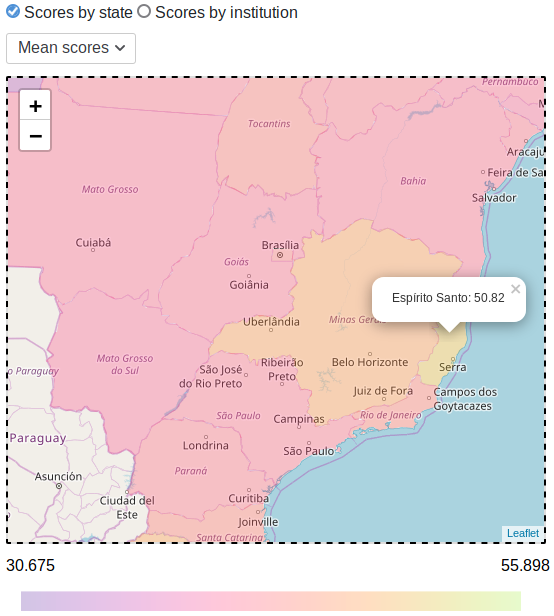
\includegraphics[width=\columnwidth]{figures/es_mean.png}
	\caption{Mean scores for the states, with Espírito Santo highlighted.}
	\label{fig:esmean}
\end{figure}

\begin{figure}
	\centering
	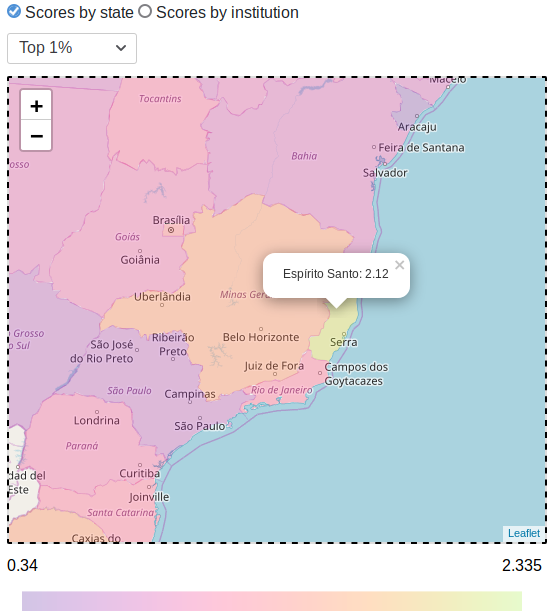
\includegraphics[width=\columnwidth]{figures/es_top.png}
	\caption{Percentages of top scores for the states, with Espírito Santo highlighted.}
	\label{fig:estop}
\end{figure}

Meanwhile, on the northeast macro-region of Brasil, which is comprised of Maranhão, Piauí, Ceará, Rio Grande do Norte, Paraíba, Pernambuco, Alagoas, Sergipe e Bahia, only two states have a value of $F_{top}$ greater than one. These states are Ceará and Rio Grande do Norte, with values of 1.52 and 1.22, respectively. Figure \ref{fig:ce} shows these two states in the context of the macro-region.

\begin{figure}
	\centering
	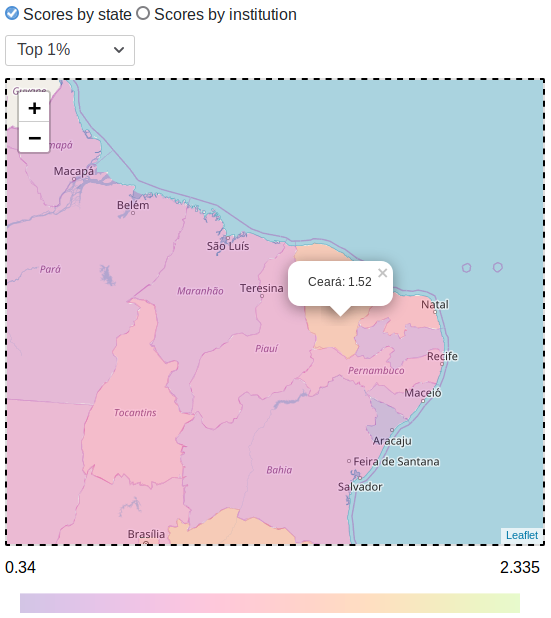
\includegraphics[width=\columnwidth]{figures/ce.png}
	\caption{Percentages of top scores for the states, with Ceará highlighted.}
	\label{fig:ce}
\end{figure}

Another interesting case is that of Paraná, which performs unexpectedly poorly when compared to the other two states of the south macro-region of Brazil. While the three states are all in the top 6 of richest states of the federation (again, in terms of GDP per capita), only Paraná has a relative percentage of bottom scores greater than one, as shown in Figure \ref{fig:pr}.

\begin{figure}
	\centering
	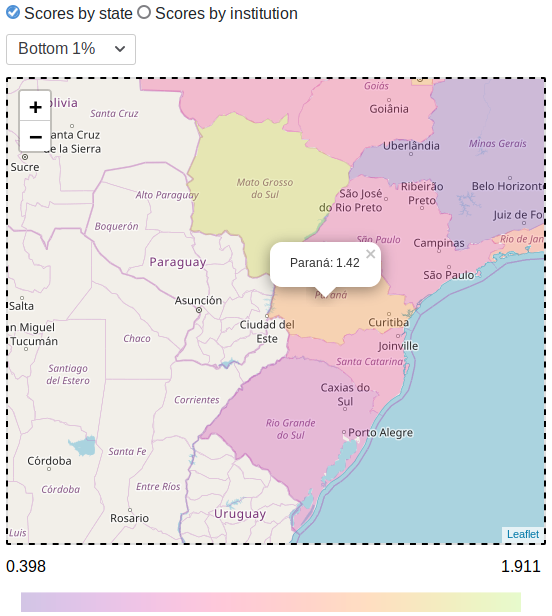
\includegraphics[width=\columnwidth]{figures/pr.png}
	\caption{Percentages of bottom scores for the states, with Paraná highlighted.}
	\label{fig:pr}
\end{figure}

\section{Conclusions}

In this work, we proposed a visualization tool for the ENADE micro-data data set, with the goal of providing users with the tools to investigate regional differences in student peformance. More specifically, we proposed two cloropleth based visualizations that allowed the users two observe the average scores and percentage of top and bottom students for each state, and also visualize how unequal was the performance of institutions within a state.

Our results show that particular factors, which we were not able to tease out with our analysis, can heavily influence the performance of students in a state, particularly when compared to similarly wealthy neighboring states. Further analysis into the cases of states like Espírito Santo, Ceará and Paraná may reveal what factors can positively or negatively influence the higher education system in a state.

\subsection{Future Work}

Given the nature of the data set investigated, there are a multitude of possible future avenues of investigation. These may include simply teasing out other interesting patterns, involving the grades, the socioeconomic factors or a combination of both. Another possibility is the development of more sophisticated visualizations, which allow for the discerning of finer details, such as details at the institution level, or visualizations which attempt to tease out patterns and groupings at the individual student level. Finally, the data also allows for the application of statistical and machine learning methods, in order to investigate correlations and causality relations between the different variables, in particular between socioeconomic variables and the performance of students.



%\bibliographystyle{abbrv}
\bibliographystyle{abbrv-doi}
%\bibliographystyle{abbrv-doi-narrow}
%\bibliographystyle{abbrv-doi-hyperref}
%\bibliographystyle{abbrv-doi-hyperref-narrow}

\bibliography{template}
\end{document}
